\documentclass[11pt,a4paper]{article}

\usepackage{graphicx}
\usepackage{url}
\usepackage{listings}
\title{Accessing IO pins of port expander(MCP23017) interfaced with R-Pi}
\author{e-Yantra Team}
\date{\today}

\begin{document}
	\maketitle
	\newpage
	\tableofcontents
	\newpage
	\section{Objective}
	In this tutorial we will learn to access IO pins of a port expander (MCP23017) interfaced with an R-Pi and will also perform some experiments with LED's, switches and LCD interfaced with this IC.
	\section{Prerequisites}
	\begin{itemize}
		\item Python programming skills 
		\item Interfacing an MCP23017 IC with an R-Pi should be known
	\end{itemize}
	
	\section{Hardware Requirement}
    \begin{enumerate}
    	\item Raspberry Pi (I will be using Version 2 Model B+)
    	\item MCP23017
    	\item Power adapter
    	\item Connecting wires
    	\item LED's
    	\item 16x2 LCD display (I will be using model JHD162A)
    	\item Push button
    	\item Resistors (330 ohms)
    	\item Potentiometer (10k ohms)
    	\item Bread board
    \end{enumerate}
    
	\section{Software Requirement}
	\begin{enumerate}
		\item PyScripter (version 2.7 or above)
		\item Mobaxterm (for windows user)
	\end{enumerate}
	
	\newpage
	\section{Theory and Description}
	
	\subsection{MCP23017}
	It is a 16 bit I/O expander with serial interface. Some of its features are:
	\begin{itemize}
		\item 16-bit remote bidirectional I/O port (I/O pins default to input)
		\item High-speed I2C interface (100 kHz, 400 kHz, 1.7 MHz)
		\item Three hardware address pins to allow up to eight devices on the bus
		\item Two pins to communicate with a master controller i.e. SCL and SDA
	\end{itemize}
	
	\begin{figure}[h!]
		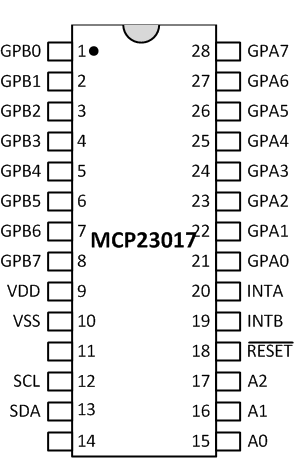
\includegraphics[scale=0.7]{mcp23017.png}
		\centering
		\caption{[5]}
	\end{figure}
	
	\flushleft
	For further information you refer the Appendix section.
	
	\subsection{Interfacing MCP23017 and detecting its address}
		In order to start programming the port expander(MCP23017) , we need to interface the IC with R-Pi in the following way:
	\begin{figure}[h!]
		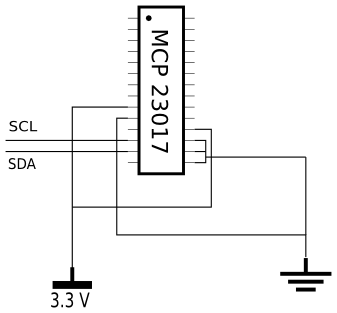
\includegraphics[scale=0.8]{interface.png}
		\centering
		\caption{[6]}
	\end{figure} 
\flushleft
			
	\begin{itemize}
			\item Connect the VDD pin and RESET on MCP23017 to 3.3v pin on an R-Pi 
			\item Connect the VSS pin on MCP23017 and A0,A1,A2 pin to GND pin on an R-Pi(If you are using 1 port expander IC then we connect the 3 address pins A0, A1 and A2 pins to GND)
			\item Connect the SCL and SDA pins from the MCP23017 IC to the respective pins on R-Pi
	\end{itemize}
				
	\vspace{0.3cm}
	\textbf{Please refer the Appendix section before making the necessary connections. }
				
	\vspace{0.3cm}
	After making all the necessary connections type the following command on the terminal \textit{sudo i2cdetect -y 1} (to see the device addresses of MCP23017 IC's interfaced )
				
	\vspace{0.3cm}
	\textbf{Note :} For a version 1 R-Pi with RAM lesser than 512MB use the command \textit{sudo i2cdetect -y 0} 
	
	
	\subsection{16x2 LCD Display}
	\vspace{0.3cm}
	LCD (Liquid Crystal Display) (JHD162A) screen is an electronic display module and find a wide range of applications. A 16x2 LCD display is very basic module and is very commonly used in various devices and circuits. These modules are preferred over seven segments and other multi segment LEDs. The reasons being: LCDs are economical; easily programmable; have no limitation of displaying special and even custom characters (unlike in seven segments), animations and so on.
	\flushleft
	A 16x2 LCD means it can display 16 characters per line and there are 2 such lines. In this LCD each character is displayed in 5x7 pixel matrix. This LCD has two registers, namely, Command and Data. The \textit{Command} register stores the command instructions given to the LCD. A command is an instruction given to LCD to do a predefined task like initializing it, clearing its screen, setting the cursor position, controlling display etc. The \textit{Data} register stores the data to be displayed on the LCD. The data is the ASCII value of the character to be displayed on the LCD. [4]
	\vspace{0.3cm}
	\textbf{Pin Diagram}
    \begin{figure}[h!]
    	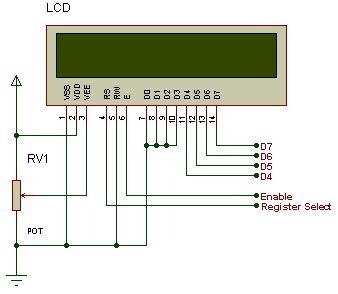
\includegraphics[scale=0.9]{lcd.png}
    	\centering
    	\caption{[5]}
    \end{figure} 
    	
	\newpage
	\flushleft
	\textbf{Pin Description }
	\vspace{0.3cm}
	
	\begin{tabular}{|c|c|c|}
		\hline
		Pin No & Function & Name \\
		\hline
		1 & Ground (0V) & Ground \\
		\hline
		2 & Supply voltage; 5V (4.7V – 5.3V) & Vcc \\
		\hline
		3 & Contrast adjustment; through a variable resistor & VEE \\
		\hline
		4 & Selects command register when low; and data register when high & Register Select \\
		\hline
		5 & Low to write to the register; High to read from the register & Read/write \\
		\hline
		6 & Sends data to data pins when a high to low pulse is given & Enable \\
		\hline
		7 & & DB0 \\
		\hline
		8 & & DB1 \\
		\hline
        9 & & DB2 \\
        \hline
		10 & 8-bit data pins & DB3 \\
		\hline
		11 & & DB4 \\
		\hline
		12 & & DB5 \\
		\hline
		13 & & DB6 \\
		\hline
		14 & &DB7 \\
		\hline
		15 & Backlight VCC (5V) & Led+ \\
		\hline
		16 & Backlight Ground (0V) & Led- \\
		\hline
	\end{tabular}
	\flushleft
	Ref: [4]
	
	
	\newpage
	\section{Experiments}
	\flushleft
	In order to program the MCP23017 chip (using I2C protocol) in Python you must install the \textbf{smbus} package. Once you have installed the package you can now start programming the chip.
    
    \vspace{0.3cm}
    \textbf{SMBus protocol commands:}
    \begin{itemize}
    	\item SMBus Read Byte:  i2c\_smbus\_read\_byte\_data()
    	This reads a single byte from a device, from a designated register.

    	
        \item SMBus Write Byte:  i2c\_smbus\_write\_byte\_data()
        
        This writes a single byte to a device, to a designated register.
        
    	
    \end{itemize}
    
	\subsection{Interfacing an LED and a Switch to R-Pi using MCP23017 IC}
     \begin{figure}[h!]
     	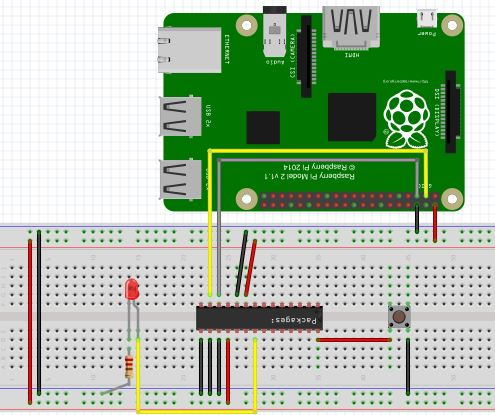
\includegraphics[scale=1]{led_switch_I2C.JPG}
     	\centering
     	\caption{[2]}
     \end{figure} 
     
     As shown in the figure:
     \begin{itemize}
     	\item Pin 9 (VDD) is connected to 5V
     	\item Pin 10 (VSS) is connected to Ground
     	\item Pin 12 (SCL) is connected to Pin 5 on the Pi GPIO
     	\item Pin 13 (SDA) is connected to Pin 3 on the Pi GPIO
     	\item Pin 18 (Reset) should be set high for normal operation so we connect this to 5V
     	\item Pins 15, 16 \& 17 (A0-A2) determine the number assigned to this device. We are only using one device so we will give it a binary zero by setting all three of these pins to 0 (ground)
     	\item Led is connected to GPA0 and switch is connected to GPA7
     \end{itemize}
    
    \newpage 
    \textbf{Code}
    \vspace{0.3cm}
    
    \lstinputlisting[language=Python]{Switch_Led_With_Mcp23017.py}
    
    \newpage 
	\subsection{Interfacing an LCD to an R-Pi using MCP23017 IC}
	\begin{figure}[h!]
		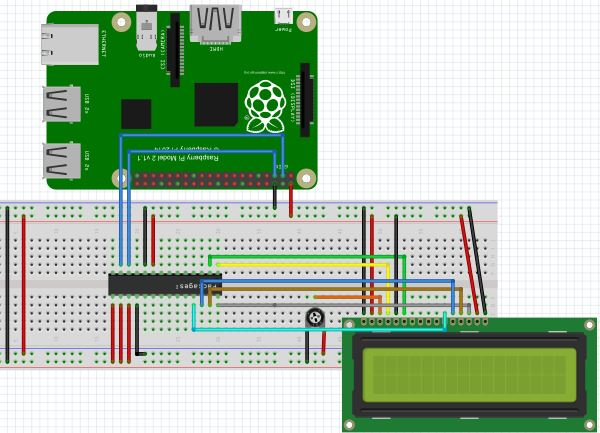
\includegraphics[scale=0.7]{LCD_I2C.PNG}
		\centering
		\caption{[2]}
	\end{figure} 
	
	 As shown in the figure:
	 \begin{itemize}
	 	\item Pin 9 (VDD) is connected to 5V (Red)
	 	\item Pin 10 (VSS) is connected to Ground (Black)
	 	\item Pin 12 (SCL) is connected to Pin 5 on the Pi GPIO 
	 	\item Pin 13 (SDA) is connected to Pin 3 on the Pi GPIO 
	 	\item Pin 18 (Reset) should be set high for normal operation so we connect this to 5V (Red)
	 	\item Pins 15, 16 \& 17 (A0-A2) determine the number assigned to this device. We are only using one device so we will give it a binary zero by setting all three of these pins to 0 (ground) (Black)
	 	\item RS and Enable pins of the LCD are connected to GPB0 and GPB1 respectively.
	 	\item R/W pin is Grounded(As it has to be used only for write operations).
	 	\item Data pins D7,D6,D5 and D4 are connected to GPA7,GPA6,GPA5 and GPA4 respectively.
	 \end{itemize}
	
	\newpage 
	\textbf{Code}
	\vspace{0.3cm}
	
	\lstinputlisting[language=Python]{Lcd_With_Mcp23017.py}
	
	\vspace{0.3cm}
	
	
	\newpage
	\section{Appendix}
	
	\subsection{Raspberry Pi 2 Pin-out Diagram}
	\begin{figure}[h!]
		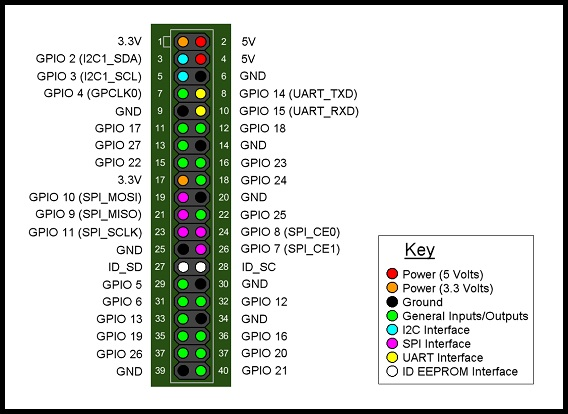
\includegraphics[scale=0.6]{RaspberryPi2_pinout.jpg}
		\centering
		\caption{[5]}
	\end{figure}
	\subsection{MCP23017 datasheet}
		
	\url{http://ww1.microchip.com/downloads/en/DeviceDoc/21952b.pdf}
	\subsection{Pinouts of MCP23017}
	\begin{figure}[h!]
		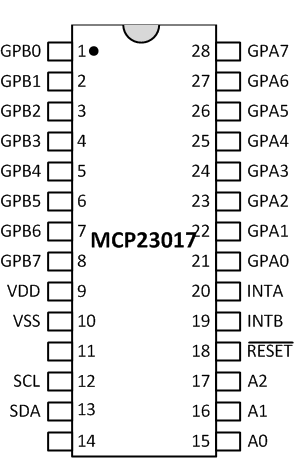
\includegraphics[scale=0.5]{mcp23017.png}
		\centering
		\caption{[5]}
	\end{figure}
			
	\newpage
	\section{References}
	\begin{enumerate}
		\item \url{https://www.kernel.org/doc/Documentation/i2c/smbus-protocol}
		\item \url{http://dangerousprototypes.com/wp-content/media/2013/04/mcp23017test_bb-600x458.png}
		\item \url{https://www.sparkfun.com/datasheets/LCD/HD44780.pdf}
		\item \url{http://www.engineersgarage.com/electronic-components/16x2-lcd-module-datasheet}
		\item \url{http://data.designspark.info/uploads/images/53bc258dc6c0425cb44870b50ab30621}
		\item \url{https://www.mathworks.com/examples/matlab/4547-add-digital-i-o-pins-to-raspberry-pi-hardware-using-mcp23017}
    \end{enumerate}
	
\end{document}



